\documentclass[12pt]{article}
\textwidth=6.35in   
\topmargin=-.05in
\oddsidemargin=0.1in
\textheight=8.45in
\headheight=15pt
\renewcommand{\baselinestretch}{1.4} %line spacing - set to 2 for doublespaced
\usepackage{graphicx} % for easy postscript figure inclusion.
\usepackage[space]{grffile}
\usepackage{url}
\usepackage{fancyhdr}
\usepackage{float}
\usepackage{authblk}
%\usepackage[sort&compress]{natbib}
%\usepackage[superscript]{cite}
\usepackage{amsmath, amsthm, amssymb}
\pagestyle{fancy}

\usepackage{xcolor}

\usepackage[
backend=biber,
style=numeric,
]{biblatex}
\addbibresource{bibliography}

\begin{document}

\pagenumbering{arabic}

\section{Introduction}


\noindent $\bigcirc$ Objective: 

\noindent $\bigstar$ Bonus: 


\section{Requirements}

\textcolor{red}{water proof ruler}

\section{Water Level Sensor}

\textcolor{red}{ https://circuitdigest.com/microcontroller-projects/interfacing-water-level-sensor-with-arduino }

Much of the information and the images for this sensor can be found on this Last Minute Engineer page\cite{LME_water_sensor}.

\begin{enumerate}
	\itemsep -1em
	\item Introduce water level sensor
	\item Discuss how they work using electrical conductivity
	\item Build circuit
	\item Program **
	\subitem Use serial comm to return and plot values
	
	\item Experiment
	\subitem Create a chart for sensor outputs based on water level
	\subitem Is the relationship linear?
	
	\item Introduce if-statements
	\subitem Can you use if-statements to make LEDs turn on/off as the water level changes?
	
	\item Use different salinity of water to mess with their systems
	
	\item Experiment
	\subitem 
	
\end{enumerate}

\subsection{How it works}

\textcolor{red}{Water is electrically conductive}

This sensor uses an electrical signal to indicate a water level. As the water in the jar rises, more and more of the sensor is going to be covered. As the sensor gets covered, it is able to output a high voltage signal. We can measure this analog voltage signal to calculate the amount of water in the jar.



\begin{figure}[H]
	\begin{center}
		%\title{}
		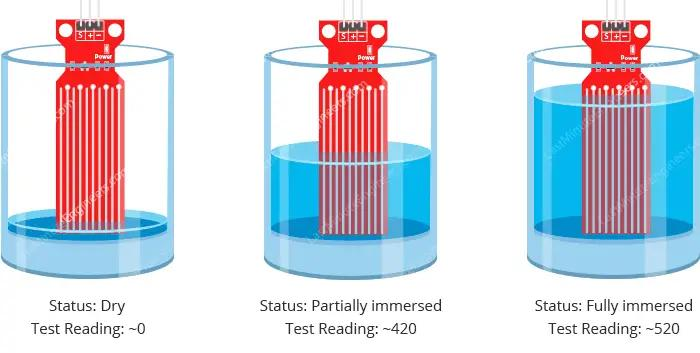
\includegraphics[scale=0.55]{Water-Level-Sensor-Calibration}
		\caption{Sensor response to different water levels.}
		\label{water_level_sensor_basics}
	\end{center}
\end{figure}









\subsection{Circuit}

The circuit for this sensor is fairly simple. All we need to do is provide a ground and power source to make it work, and then a connect a wire from the sense pin on the sensor to an analog pin on the Arduino.

Metal, like the contact strips on our sensor, will start to rust or corrode when it is exposed to water. The corrosion of a metal can occur much faster if an electrical current is flowing while it is exposed to water. As a result, we will be powering our sensor using a digital pin. We will turn on the power when we want to take a measurement and then switch it off when we are not using it.



\begin{figure}[H]
	\begin{center}
		%\title{}
		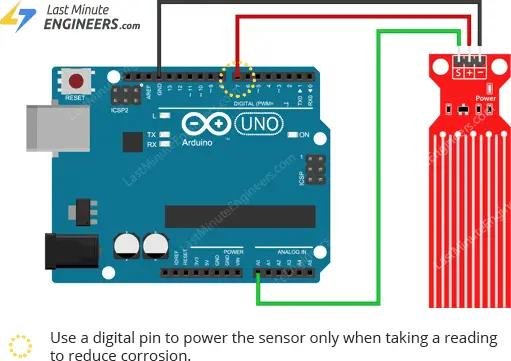
\includegraphics[scale=0.55]{circuit_water_sensor_basic}
		\caption{Sensor response to different water levels.}
		\label{circuit:water_sensor_basic}
	\end{center}
\end{figure}














\subsection{Program}

Here is the program that we will be using to collect measurements. The main loop is quite simple.

\begin{enumerate}
	\itemsep -1em
	\item Collect a measurement for the level of the water.
	\item Send the measurement to the computer.
	\item Delay until it time to take the next measurement.
\end{enumerate}

The more complicated part is the process to obtain a measurement. This is done using the function \textbf{\textit{ measure\_water\_level}}.

\begin{enumerate}
	\itemsep -1em
	\item Turn digital pin 7 on, this provides power to the sensor.
	\item Wait for 10 milliseconds, allowing the sensor time to settle after the power has been turned on.
	\item Make a measurement for the level of the water.
	\item Turn off pin 7, switching off the power to the sensor to protect it.
	\item Return the measurement.
\end{enumerate}



\textcolor{red}{update caption}

\begin{figure}[H]
	\begin{center}
		%\title{}
		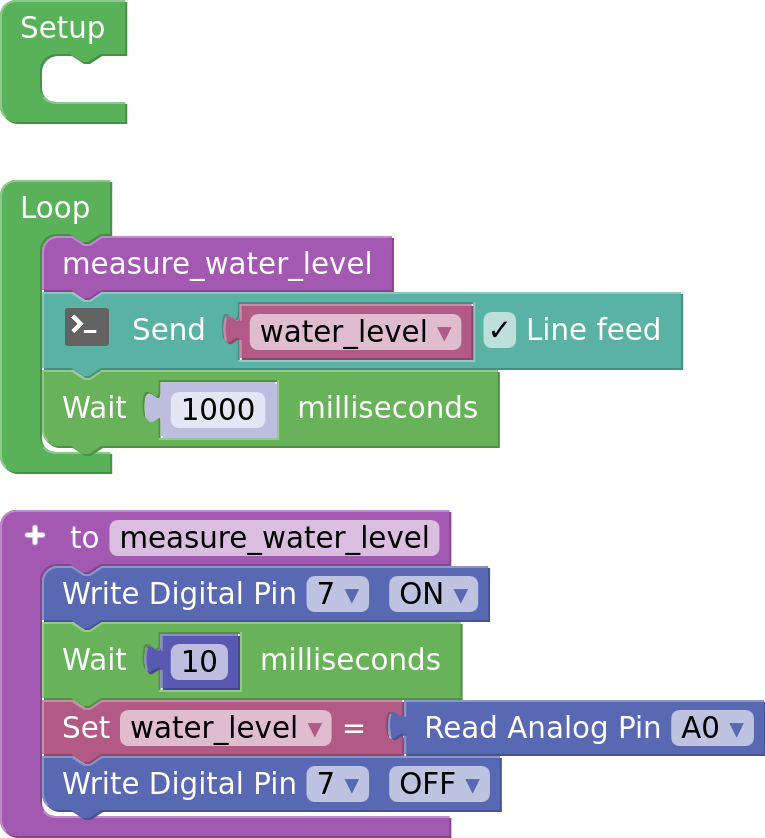
\includegraphics[scale=0.3]{p_water-level-sensor}
		\caption{Sensor response to different water levels.}
		\label{p:water_sensor_simple}
	\end{center}
\end{figure}













\subsection{Experiment}

For some of the following tasks that we will be doing, we need to know what the sensor's output is for a range of different water levels. Start with an empty cup and record the sensor's output. Using a ruler, add water to raise the water level 5mm. Rec

\begin{enumerate}
	\itemsep -1em
	\item Start with an empty cup and record the sensor's output.
	\item Using a ruler, add water to raise the water level 5mm.
	\item Record the new measurement from the sensor.
	\item Repeat steps 2 \& 3 until the sensor is fully covered. Try not to get water on the electronics at the top of the sensor if possible.
\end{enumerate}



\noindent $\bigcirc$ Objective: Create a chart of the sensor's output for a range of different water levels in the cup. You can use Google Spreadsheets to record your results.

\noindent $\bigstar$ Bonus: 








\subsection{If Statements}

\subsubsection{Objective}

For this part, we will be adding LEDs to your circuit. The goal of the LEDs is to have then turn on when the water reaches specific levels. You can use the results from the previous experiment to decide which at what measurement value each LED should turn on/off.

Connect a green LED to pin 9, yellow to 10, and red to pin 11. Remember, you always have to use a resistor with LEDs. You can reference last weeks notes if you forget how to connect LEDs in a circuit.

\subsubsection{If/Else Flow Control}

To make the LED turn on/off depending on the level of the water we will require a new type of programming logic flow control with \textbf{\textit{if/else statements}}. They work using the following flow: \textbf{\textit{if}} some condition is true then \textbf{\textit{do}} some action, \textbf{\textit{else}} do something else. Look at figure \ref{p:water_sensor_if_else} and look for the bold \& italics terms in the program.


\subsubsection{Program}

We will need to add a new function for each LED. An example is provided below for the first LED. You will need to make a new function for each of the other LEDs. The new function uses an if/else statement. This function, \textbf{\textit{set\_low\_level\_led}}, with have the following flow:

\begin{enumerate}
	\itemsep -1em
	\item \textbf{\textit{if}} the water level measurement exceeds the value 300, then
	\begin{itemize}
		\item \textbf{\textit{do}}, turn on pin 9 to light up the LED
	\end{itemize}
	\item \textbf{\textit{else}}, turn off pin 9 to switch off the LED
\end{enumerate}

\noindent Note: the value used here is 300. It was chosen as a random example and you will need to change it based on the experimental results you obtained in the previous section.

\textcolor{red}{update caption}

\begin{figure}[H]
	\begin{center}
		%\title{}
		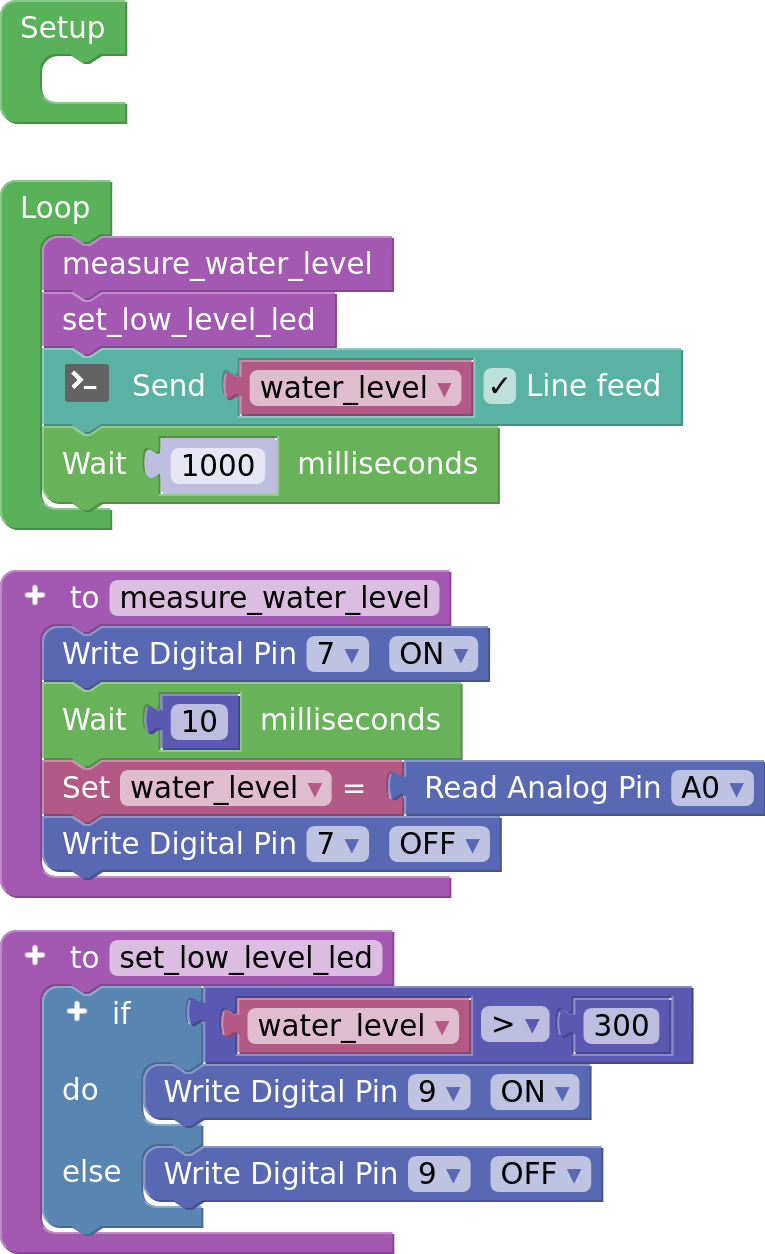
\includegraphics[scale=0.3]{p_water-level-sensor_if-else}
		\caption{Sensor response to different water levels.}
		\label{p:water_sensor_if_else}
	\end{center}
\end{figure}


\subsubsection{Your Turn}

\noindent $\bigcirc$ Objective: Add 3 LEDs to your circuit: a green, yellow and red one. Make the LEDs turn on only when:
\begin{enumerate}
	\itemsep -1em
	\item Green - the cup is $1/4$ full or more
	\item Yellow - the cup is $1/2$ full or more
	\item Red - the cup is $3/4$ full or more
\end{enumerate}

\noindent $\bigstar$ Bonus (A big challenge!): Can you make the LEDs progressively light over their ranges? You will need to use the map function and PWM output to make this work. For example, the yellow LED should remain fully off until the green LED is at full brightness when the cup is $1/4$ full. Then, as the cup fills up from $1/4 \rightarrow 1/2$, the yellow LED should progressively get brighter and brighter.



\subsubsection{Testing the System}

We will be testing your results to see how it performs!








\section{Line Detector}

https://circuitdigest.com/microcontroller-projects/interfacing-ir-sensor-module-with-arduino




\subsection{How it works}

\subsection{Circuit}

\subsection{Program}

\subsection{Experiment}





\section{Ultra-Sonic Range Finder}

https://circuitdigest.com/microcontroller-projects/interfacing-hcsr04-ultrasonic-sensor-module-with-esp32




\subsection{How it works}

The ultrasonic sensor is capable of measuring distances between 2 cm and 400 cm (4 meters). It does this by emitting a short sound wave and listening for an echo. The duration of time between the initial sound pulse and the echo can be used to determine how far away the object is.

\subsection{Circuit}

\subsection{Program}

\subsection{Experiment}






\newpage
%\bibliographystyle{numeric}
%\bibliography{bibliography}

\printbibliography


%\begin{thebibliography}{1}
	
%	\bibitem{LME water sensor} https://lastminuteengineers.com/water-level-sensor-arduino-tutorial/

%\end{thebibliography}

\end{document}




 




%Outline for function calls

%\begin{figure}[H]
%\begin{center}
%\title{}
%\includegraphics[scale=0.7]{HallEffect}
%\caption{Diagram showing current flow and build up of charge due to electric and magnetic %fields.\cite{Fitzpatrick}}
%\label{fig:pic}
%\end{center}
%\end{figure}

%\begin{equation} \label{eq:Lorentz}
%\vec{F}=q(\vec{E}+\vec{v} \times \vec{B})
%\end{equation}

%\cite{memoir}
%\ref{eq:Lorentz}

%\bibitem{memoir} Bridgman, P. W. "Biographical Memoir of Edwin Herbert Hall." BIOGRAPHICAL MEMOIRS (n.d.): 79-82.  \url{http://www.nasonline.org/publications/biographical-memoirs/memoir-pdfs/hall-edwin.pdf}. Web. 11 Apr. 2015.
